\chapter{System architecture}
\label{sec:sys-architecture}


\section{Hardware architecture}
Choosing the right components is essential for keeping cost low and meeting the requirements for the system. Therefore it is important to have a well thought out hardware architecture. 

\subsection{Overview}
The Boat autopilot system can be broken down in to two parts a User interface and then controller.
The controller can be broken down even more. It can be split up into a programmable controller, actuators and sensors, and some components to bind this together.

The programmable controller need a WiFi and Ethernet interface to communicate with the user interface. it also need an interface to communicate with sensors and actuators. 

Since the only sensor in this version of the Boat autopilot is a GPS, we only need a serial UART interface, which is the standard if the GPS uses the NMEA protocol. 

The actuators in the system are motors that can be controlled by Pulse width modulation, and so PWM is the protocol used to control the actuators. Motors cant run off of the low amperage of a controller, therefore a motor controller is required, which can take a low voltage PWM signal and step it up to higher voltage. It also has to be able to deliver the required amount amperage of the motor. 

To power the system a battery is required and to use it all over the system a power regulator is a good idea, since motors, sensors and the controller require different voltages.

\subsubsection{General BDD}

To get an overview of the different part of the system a block definition diagram (BDD) has been drawn up.
In figure \ref{fig:general_bdd} the system blocks can be seen. There is the entire system Boat autopilot, which is broken down in to 2 parts Captain and User Interface. The User interface is what the user interacts with to control the system. It need a WiFi and/ or Ethernet connection to talk with the Captain part. Captain requires a WiFi and/or a Ethernet connection to the User Interface, it also need a battery, a 8.4 volt battery has been chosen. 

Captain can be broken down in to further parts, A Controller, Power regulator, Motor Controller, Motor, and GPS.
The Controller is a programmable controller, with a WiFi and Ethernet adapter, it is responsible for controlling the other parts of Captain. It has a 5 V input to power it, and outputs a 3.3 V output to power the GPS, from the GPS it gets a serial UART signal in the form of NMEA protocol. It also output 1 to 2 PWM signal to 1 to 2 Motor Controllers which drive 1 to 2 Motors.

To power all the parts a Power regulator is need, it takes the battery voltages and steps it down to 5 V for the controller, and passes 8.4 V to the motor controller.

\begin{figure}[H]
	\centering
	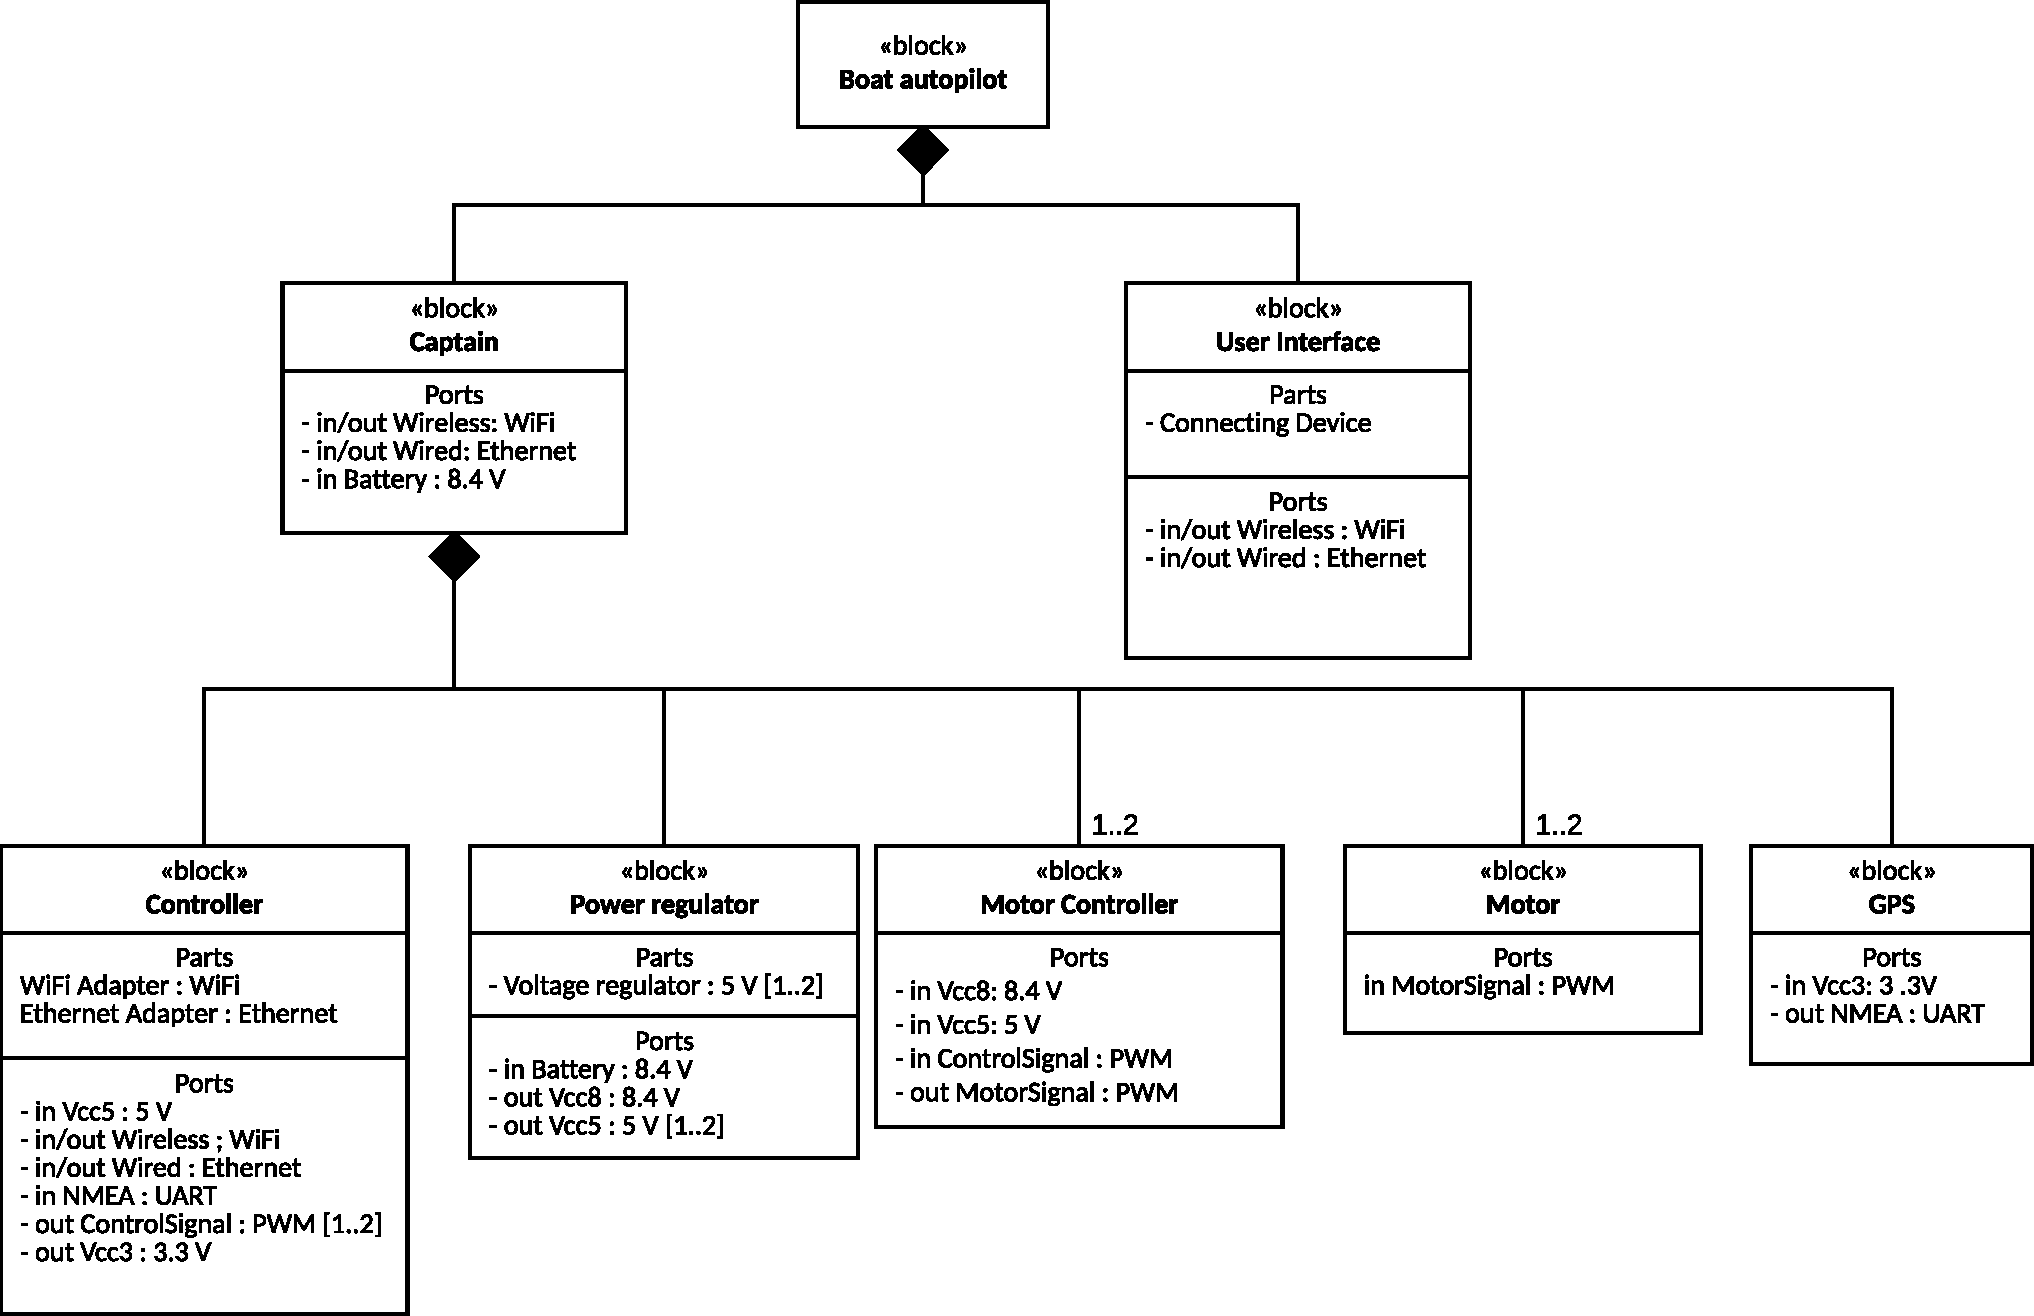
\includegraphics[width=1\linewidth]{Images/System_architecture/General_BDD}
	\caption{General BDD}
	\label{fig:general_bdd}
\end{figure}

To further describe the system a internal block diagram or IBD can be drawn, figure \ref{fig:general_ibd}, it describes the connections of the blocks from the BDD in figure \ref{fig:general_bdd}. 

Every block from the BDD gets and box, and inside a box is all of its blocks. On the edge of the blocks there are arrow indicating how the signals of the system correspond to each other.

\subsubsection{General IBD}
\label{sec:general_ibd}
\begin{figure}[H]
	\centering
	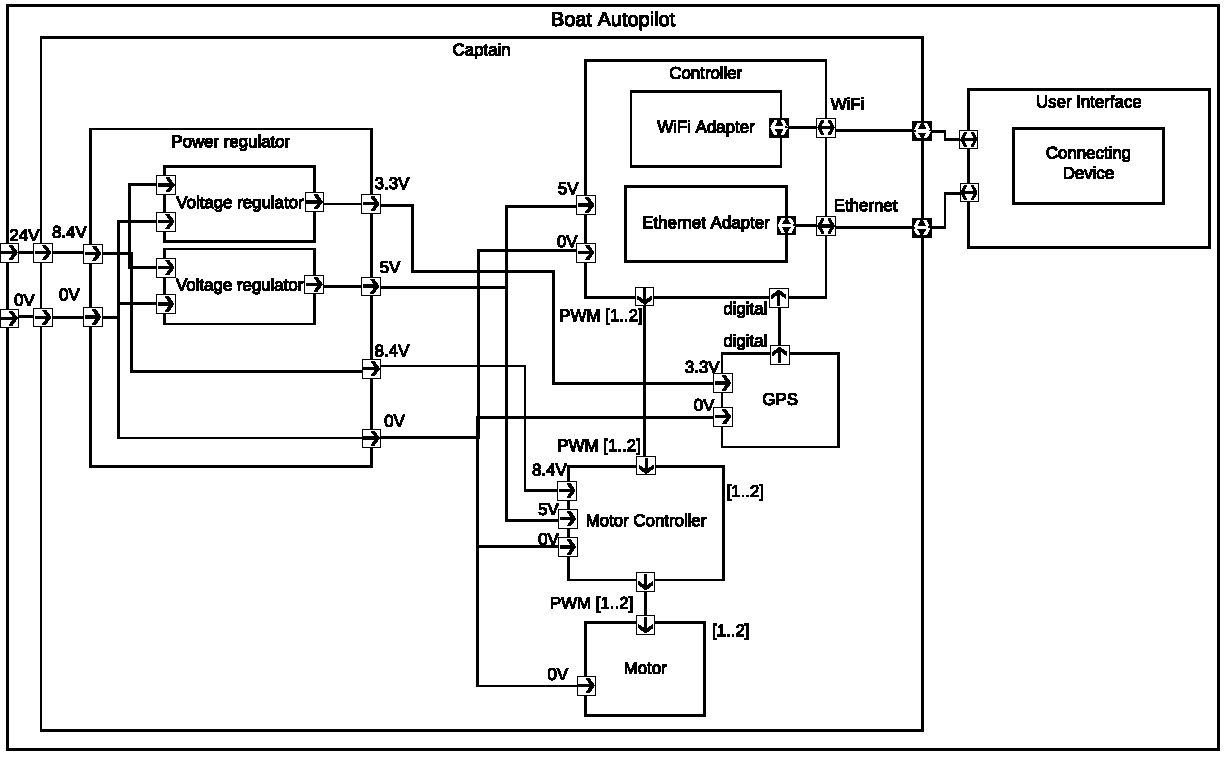
\includegraphics[width=1\linewidth]{Images/System_architecture/General_IBD}
	\caption{General IBD}
	\label{fig:general_ibd}
\end{figure}

\paragraph{Signal list}


Table~\ref{table:general_ibd} shows the signal list for the system, and a description
\begin{table}[htbp]
	\centering
	\begin{tabular}{|l|l|l|}
		\hline
		\textbf{Signal type} 	&\textbf{Name}		&\textbf{Description} \\\hline
		8.4V			&Battery	&8.4V supply from a battery\\\hline
		
		8.4V			&Vcc8		&8.4V supply to Motor Controller\\\hline
		5V			&Vcc5		&5V supply to Controller and Motor Controller\\\hline
		3.3V			&Vcc3		&3.3V supply to GPS\\\hline
		0V			&0V			&System ground\\\hline
		PWM	&ControlSignal	&PWM-signal to Motor Control, 5V\\\hline
		PWM	&MotorSignal	&PWM-signal to Motor, 8.4V\\\hline
		UART		&NMEA		&GPS data to Controller through serial UART\\\hline	
		WiFi		&WiFi		&WiFi signal between Controller and User interface\\\hline
		Ethernet	&Ethernet	&Ethernet signal between Controller and User interface\\\hline
		
		
	\end{tabular}
	\caption{Signal list for General IBD}
	\label{table:general_ibd}
\end{table}

\paragraph{PWM}
Pulse with modulation is a technique of modulating a digital signal, so it appears to to have different amplitudes to a slow system, for example a motor. This is done by switching the signal on and off with a defined frequency, but changing the duty cycle. The duty cycle is the amount of time the signal is on in a given period.\cite{PWM}

\paragraph{NMEA}
The NMEA is a protocol described by National marine electronics association. And is the standard used for most GPS systems, it sends it data over a serial UART connection. \cite{NMEA}

\paragraph{WiFi}
WiFi is a wireless local area network standard defined be IEEE\cite{WIFI}. It is used for communication between different devices on a local network or ad-hoc, meaning a device hosts a network for other devices to connect to. 

\paragraph{Ethernet}
Ethernet is a wired communication standard defined be IEEE\cite{ethernet}. In this system it is used in the same way as WiFi, to let different devices communicate.

\section{Software architecture}
\label{sec:soft-architecture}
Software architecture is in this project used to get an overview of how the different parts of the system are going to interact.
This means defining a domain model, application model and a many sequence diagrams. 

A domain model figure \ref{fig:domain_model} can be used to describe the boundaries of a system, where does the user interact and should the system respond. I the case of CAPTAIN we have 2 actors, the Technician and the User. The technicians goal when using the system is to set it up, by entering various parameters and settings into the system that result in a working autopilot, these settings could be for example be PID controller terms. The Interface in this case a web interface should then tell the rest of the system about these changes.

The technician is not the actor who operates the system generally, that would be the user. The users goal is to get the boat to move in certain ways. This is done through the web interface, where there is the ability to run different modes, including stopping the boat. the user can also get feedback from the system from the web interface.

When the web interface gets commands from the user it save the necessary data. Then it sends commands to the controller, which is in charge of calculating the path the boat should take. It is also controlling the motors.They then move the boat to a new position, this new position i sensed by the GPS.the controller gets this new position from the GPS and is able to tell the motors where to go next.

The current position, calculated path and other status related information, is send from the controller to the Web interface, where the user can then observe it and take appropriate actions.

\begin{figure}[h]
	\centering
	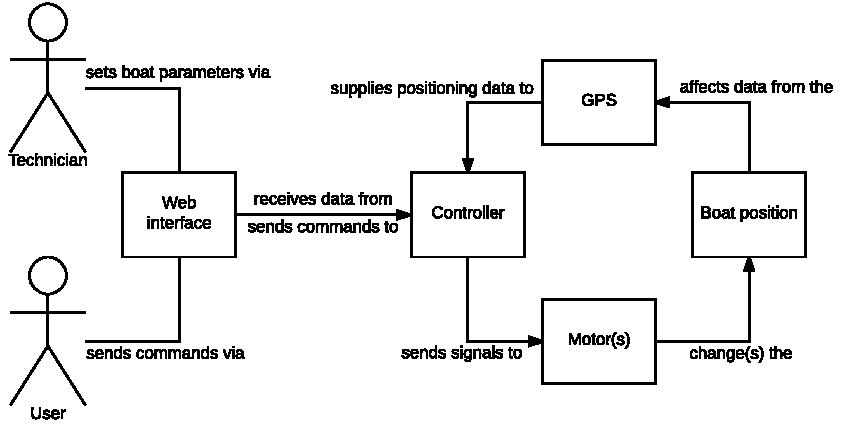
\includegraphics[width=1\linewidth]{Images/System_architecture/Domain_Model}	
	\caption{Domain Model}
	\label{fig:domain_model}
\end{figure}

From the domain model and use cases, an application model can be devised, see figure \ref{fig:appliction_model}. From the domain model there can be extracted three types of elements; boundary, control and entity.
a boundary is some sort of interface to the real world, in CAPTAIN this is the web interface, motor(s) and the GPS. Then there is the control which is the Controller, this is responsible for the flow between boundaries and entities. 

From the use cases the functionality of the the four elements can be described:
The web interface is has responsibility in three areas; profiles, diagnostics, navigation.
The profiles responsibility includes:
\begin{itemize}
\item Creating new parameter profiles
\item Delting parameter profiles
\item Editing parameter profiles
\item Displaying parameter profiles
\item Setting an active parameter profile
\item Displaying the active parameter profile
\end{itemize}
The diagnostics responsibility includes:
\begin{itemize}
\item Requesting diagnostics data from the controller
\item Getting connection diagnostics data.
\end{itemize}
Finally the navigation responsibility includes:
\begin{itemize}
\item Defining a point to point destination
\item Defining a coverage rectangle
\item Displaying data on a map
\item Displaying coordinates
\item Telling the controller to calculate a point to point path
\item Telling the controller to calculate a coverage rectangle path
\item Display a path from the controller
\item Display the postion and orientation of the boat
\item Telling the controller to run a path
\item Telling the controller to stop the boat
\end{itemize}
The controller is responsible for:
\begin{itemize}
\item Setting the the parameters from the active profile
\item Getting diagnostics from different parts of the system
\item Calculating the point to point path
\item Calculating the coverage path
\item Calculating the estimated time enroute
\item Run the boat, steer according to GPS and path
\item Stop the boat
\end{itemize}

The GPS is responsible for, getting the gps data, and its own diagnostics data.

Finally the motor(s) are responsible for setting and getting the thrust of the actual motors.

\begin{figure}[h]
	\centering
	\includegraphics[width=1\linewidth]{Images/System_architecture/Application_Model}
	\caption{Application Model}
	\label{fig:appliction_model}
\end{figure}

With the functionality of the elements defined, sequence diagrams have been created to illustrate the flow of the different functions, in relation to the use cases.

In figure \ref{fig:seq:uc1} a technician actor creates a new parameter profile, and the web interface responds by displaying a default parameter profile back to the technician.

\begin{figure}[H]
	\centering
	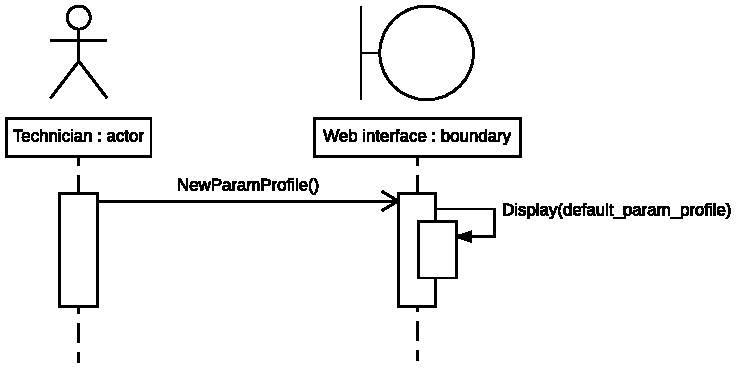
\includegraphics[width=0.8\linewidth]{Images/System_architecture/Use_case_1_SD}
	\caption{Sequence diagram for Use case 1 - New parameter profile}
	\label{fig:seq:uc1}
\end{figure}

In figure \ref{fig:seq:uc2} a technician actor deletes a selected parameter profile.

\begin{figure}[H]
	\centering
	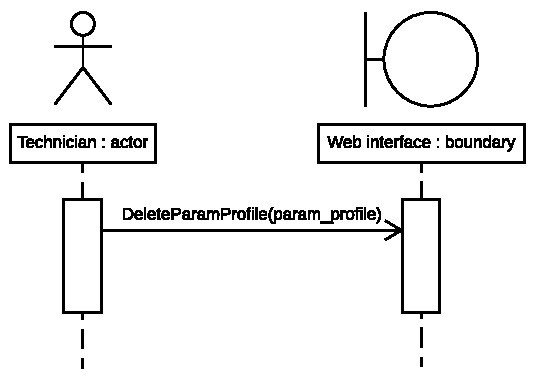
\includegraphics[width=0.7\linewidth]{Images/System_architecture/Use_case_2_SD}
	\caption{Sequence diagram for Use case 2 - Delete parameter profile}
	\label{fig:seq:uc2}
\end{figure}

In figure \ref{fig:seq:uc2} a technician actor wants edit an parameter profile so first the parameter profile is displayed to the on the web interface. Next the technician edits the parameter profile with some parameters.

\begin{figure}[H]
	\centering
	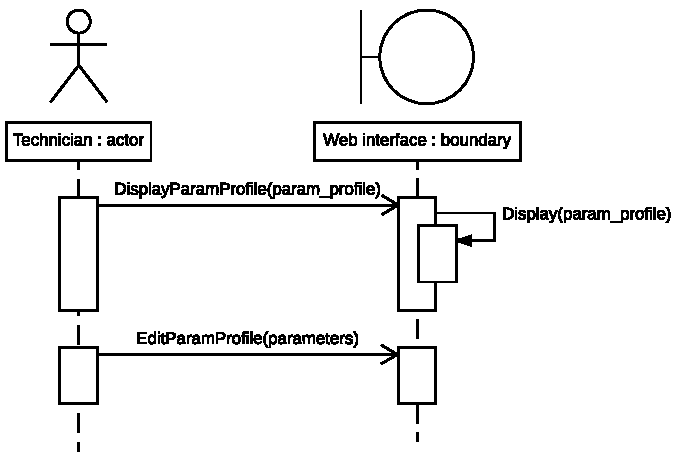
\includegraphics[width=1\linewidth]{Images/System_architecture/Use_case_3_SD}
	\caption{Sequence diagram for Use case 3 - Edit parameter profile}
	\label{fig:seq:uc3}
\end{figure}

In figure \ref{fig:seq:uc4} a technician actor wants to set a parameter profile as the currently active one, this is done by setting a selected parameter profile active, the web interface displays the active parameter profile, and sends the active parameter profile to the controller

\begin{figure}[H]
	\centering
	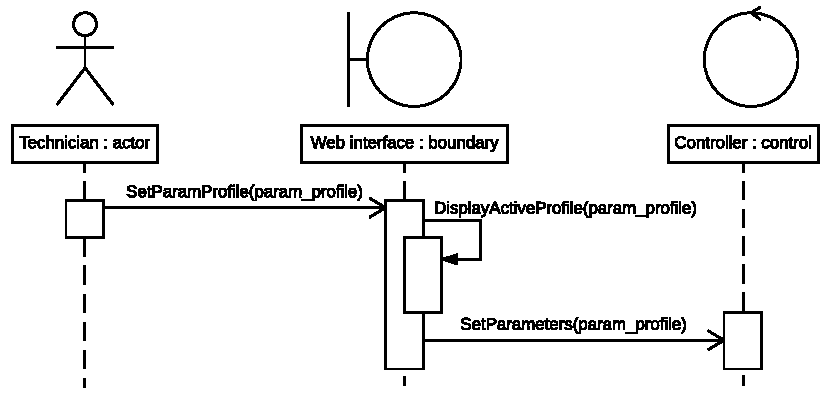
\includegraphics[width=1\linewidth]{Images/System_architecture/Use_case_4_SD}
	\caption{Sequence diagram for Use case 4 - Set active parameter profile}
	\label{fig:seq:uc4}
\end{figure}

In figure \ref{fig:seq:uc5} a user or technician actor Request diagnostics from web interface. The interface responds by asking the controller for diagnostics. The controller then gets; the speed of the thruster(s), the GPS data, and GPS diagnostics. Then the controller ask the web interface for connection diagnostics. Once all of the data is gathered it is all returned to the web interface, which then displays the diagnostics and the boats position on a map.

\begin{figure}[H]
	\centering
	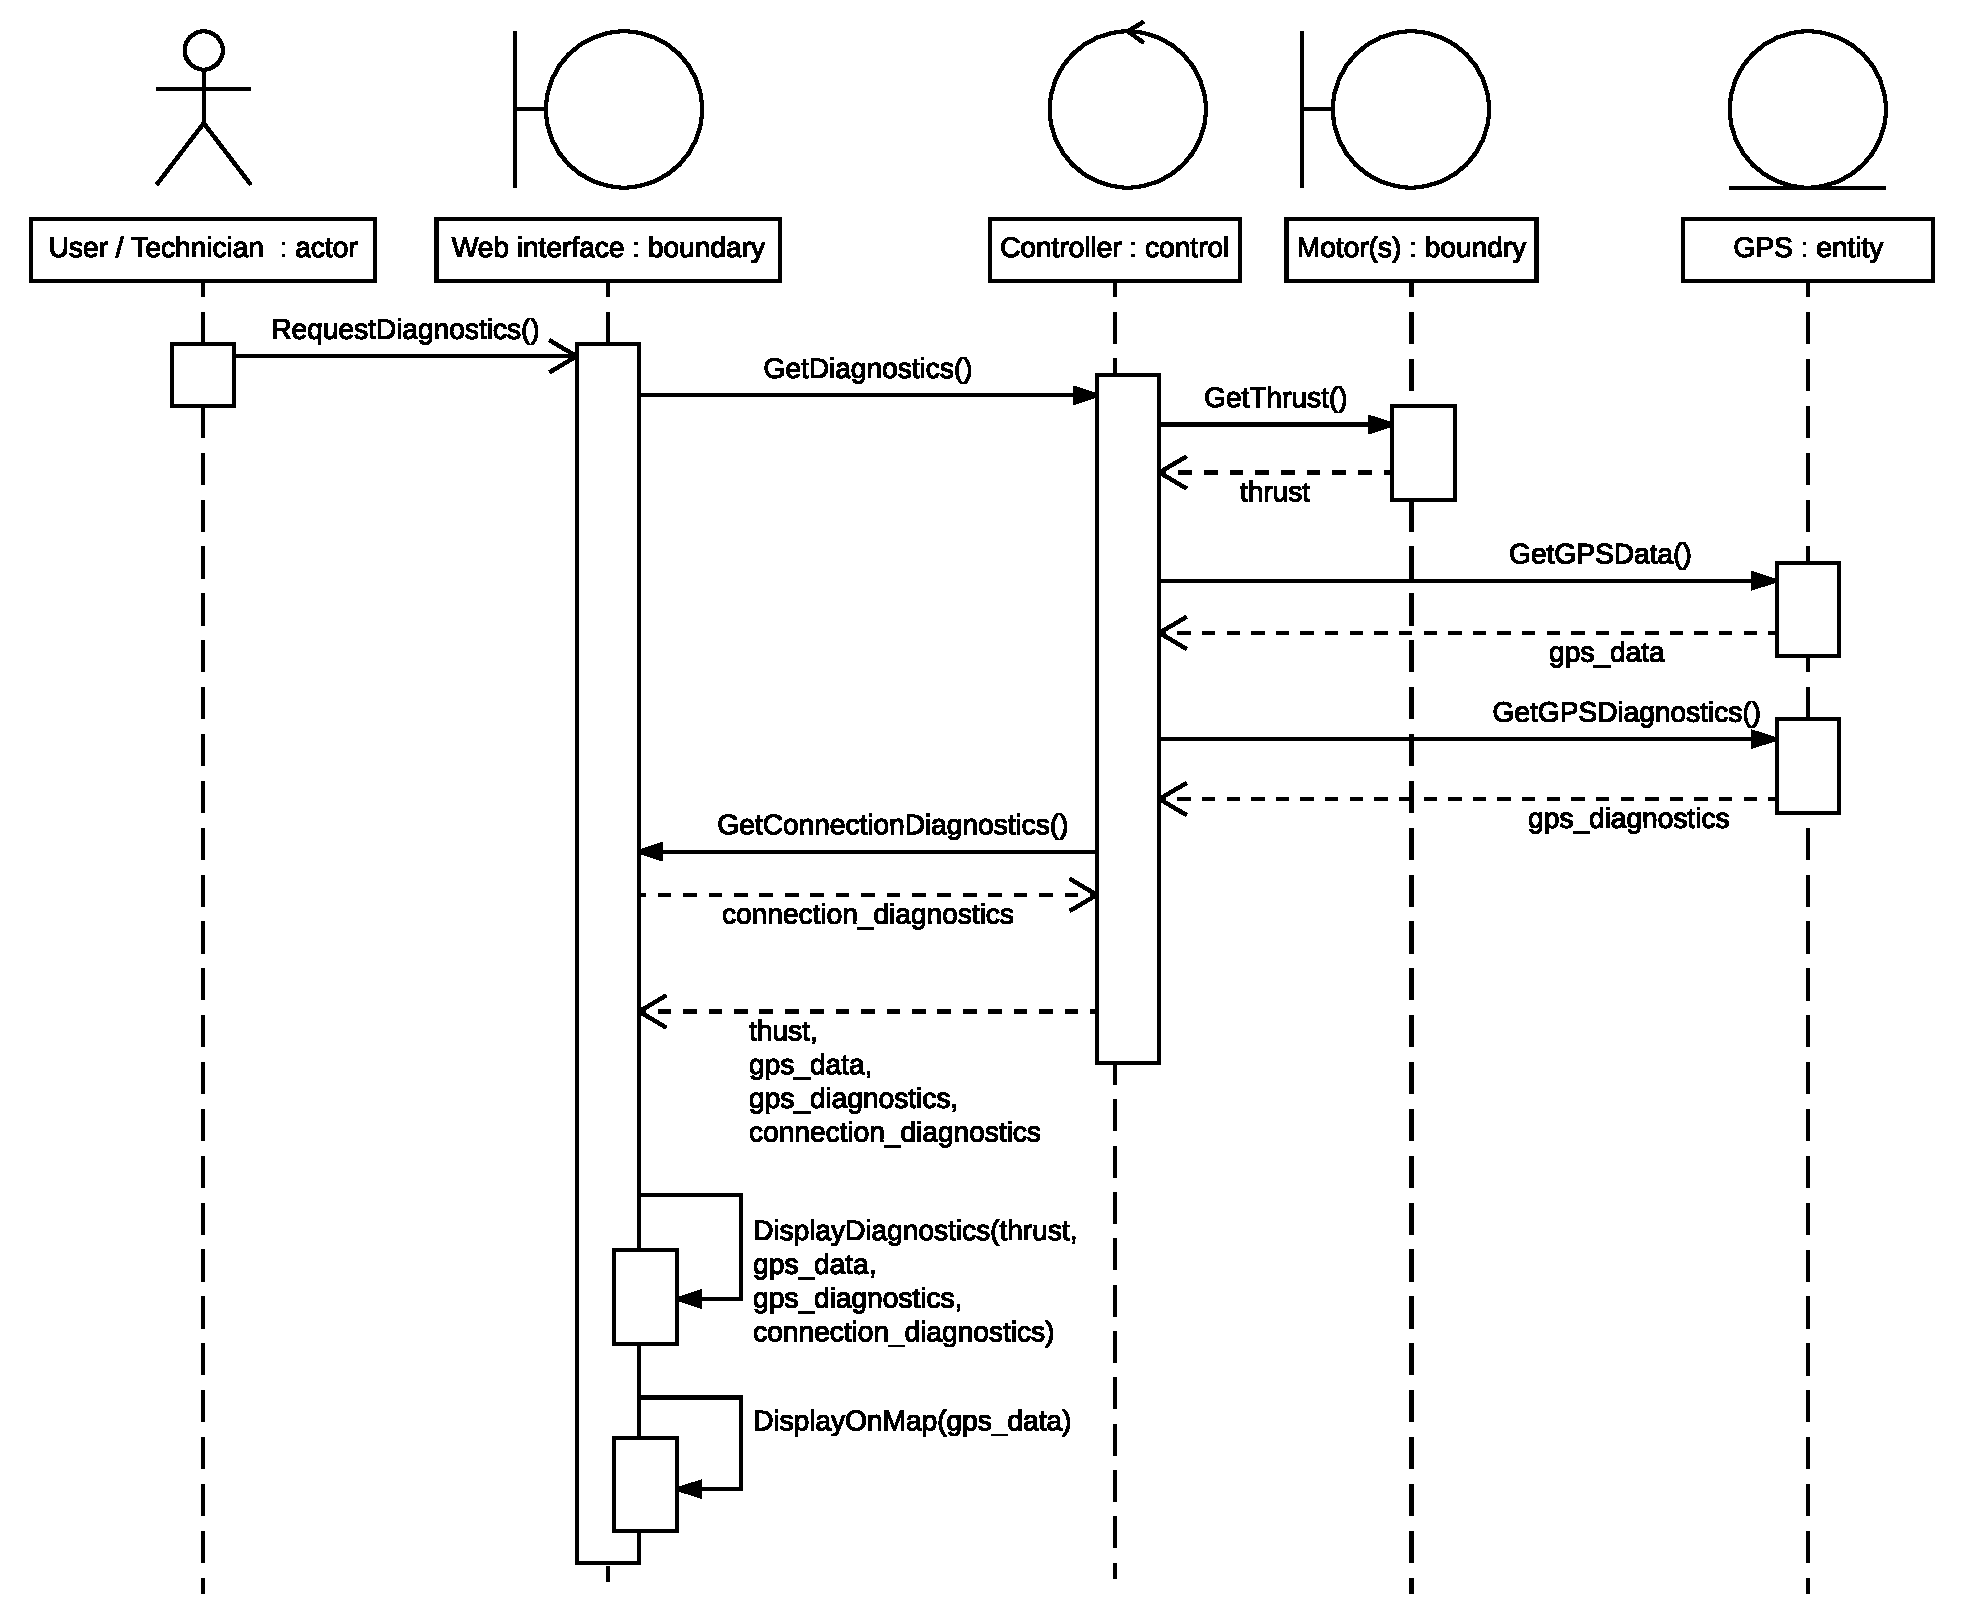
\includegraphics[width=1\linewidth]{Images/System_architecture/Use_case_5_SD}
	\caption{Sequence diagram for Use case 5 - Request diagnostics}
	\label{fig:seq:uc5}
\end{figure}

in figure \ref{fig:seq:uc6} a user actor sets a destination for a point to point operation. the coordinate of the destination is then displayed on the map as well as displaying it as text.

\begin{figure}[H]
	\centering
	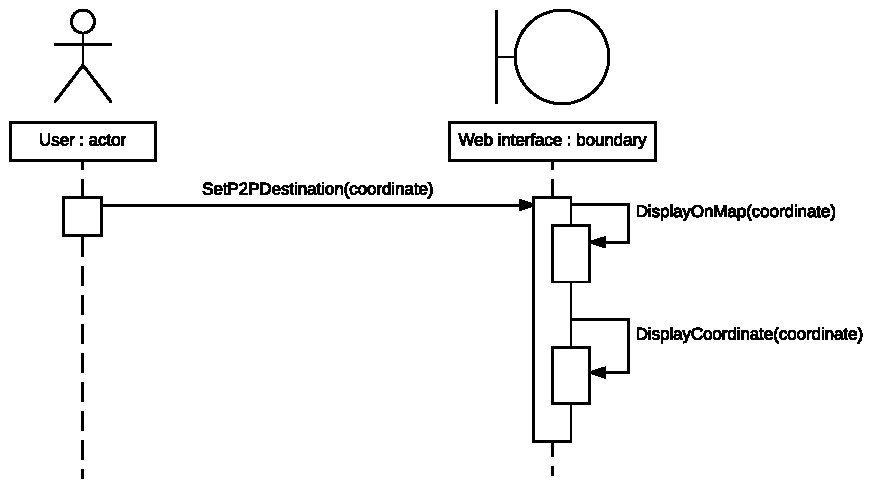
\includegraphics[width=1\linewidth]{Images/System_architecture/Use_case_6_SD}
	\caption{Sequence diagram for Use case 6 - Set point to point destination}
	\label{fig:seq:uc6}
\end{figure}

In figure \ref{fig:seq:uc7} a user actor wants to calculate a point to point path, and the user has already selected a destination. The web interface asks the controller to calculate a path with the coordinate specified by the user. The controller get the GPS data and calculates a line from the boat position to the destination and returns it to the web interface. The web interface then displays this path.

\begin{figure}[H]
	\centering
	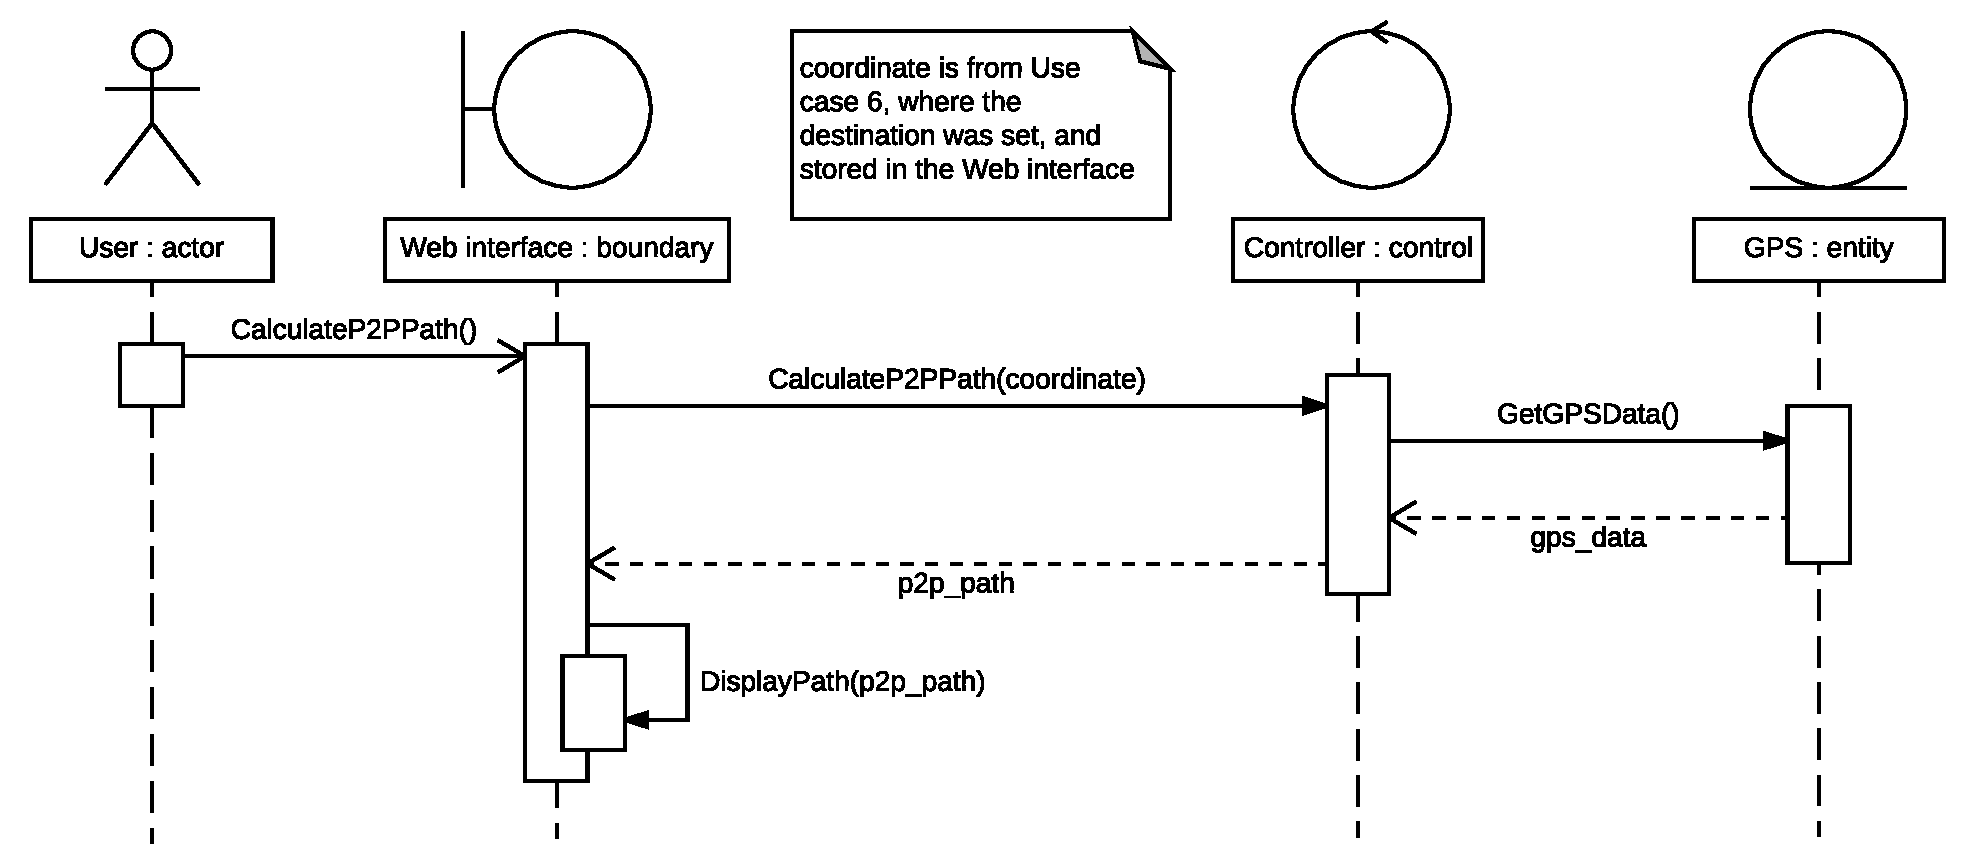
\includegraphics[width=1\linewidth]{Images/System_architecture/Use_case_7_SD}
	\caption{Sequence diagram for Use case 7 - Calculate point to point path}
	\label{fig:seq:uc7}
\end{figure}

In figure \ref{fig:seq:uc8} a user actor wants to run the a point to point path. Before this can be done, first the user must have calculated a path. The web interface tells the controller to run the point to point path previously calculated. The controller now gets the GPS data, and set the thruster(s) accordingly, it then displays the GPS data on the web interface. Then it calculates the estimated time enroute, to display on the web interface. Everything from getting the GPS data is repeated until the destination is reached.

\begin{figure}[H]
	\centering
	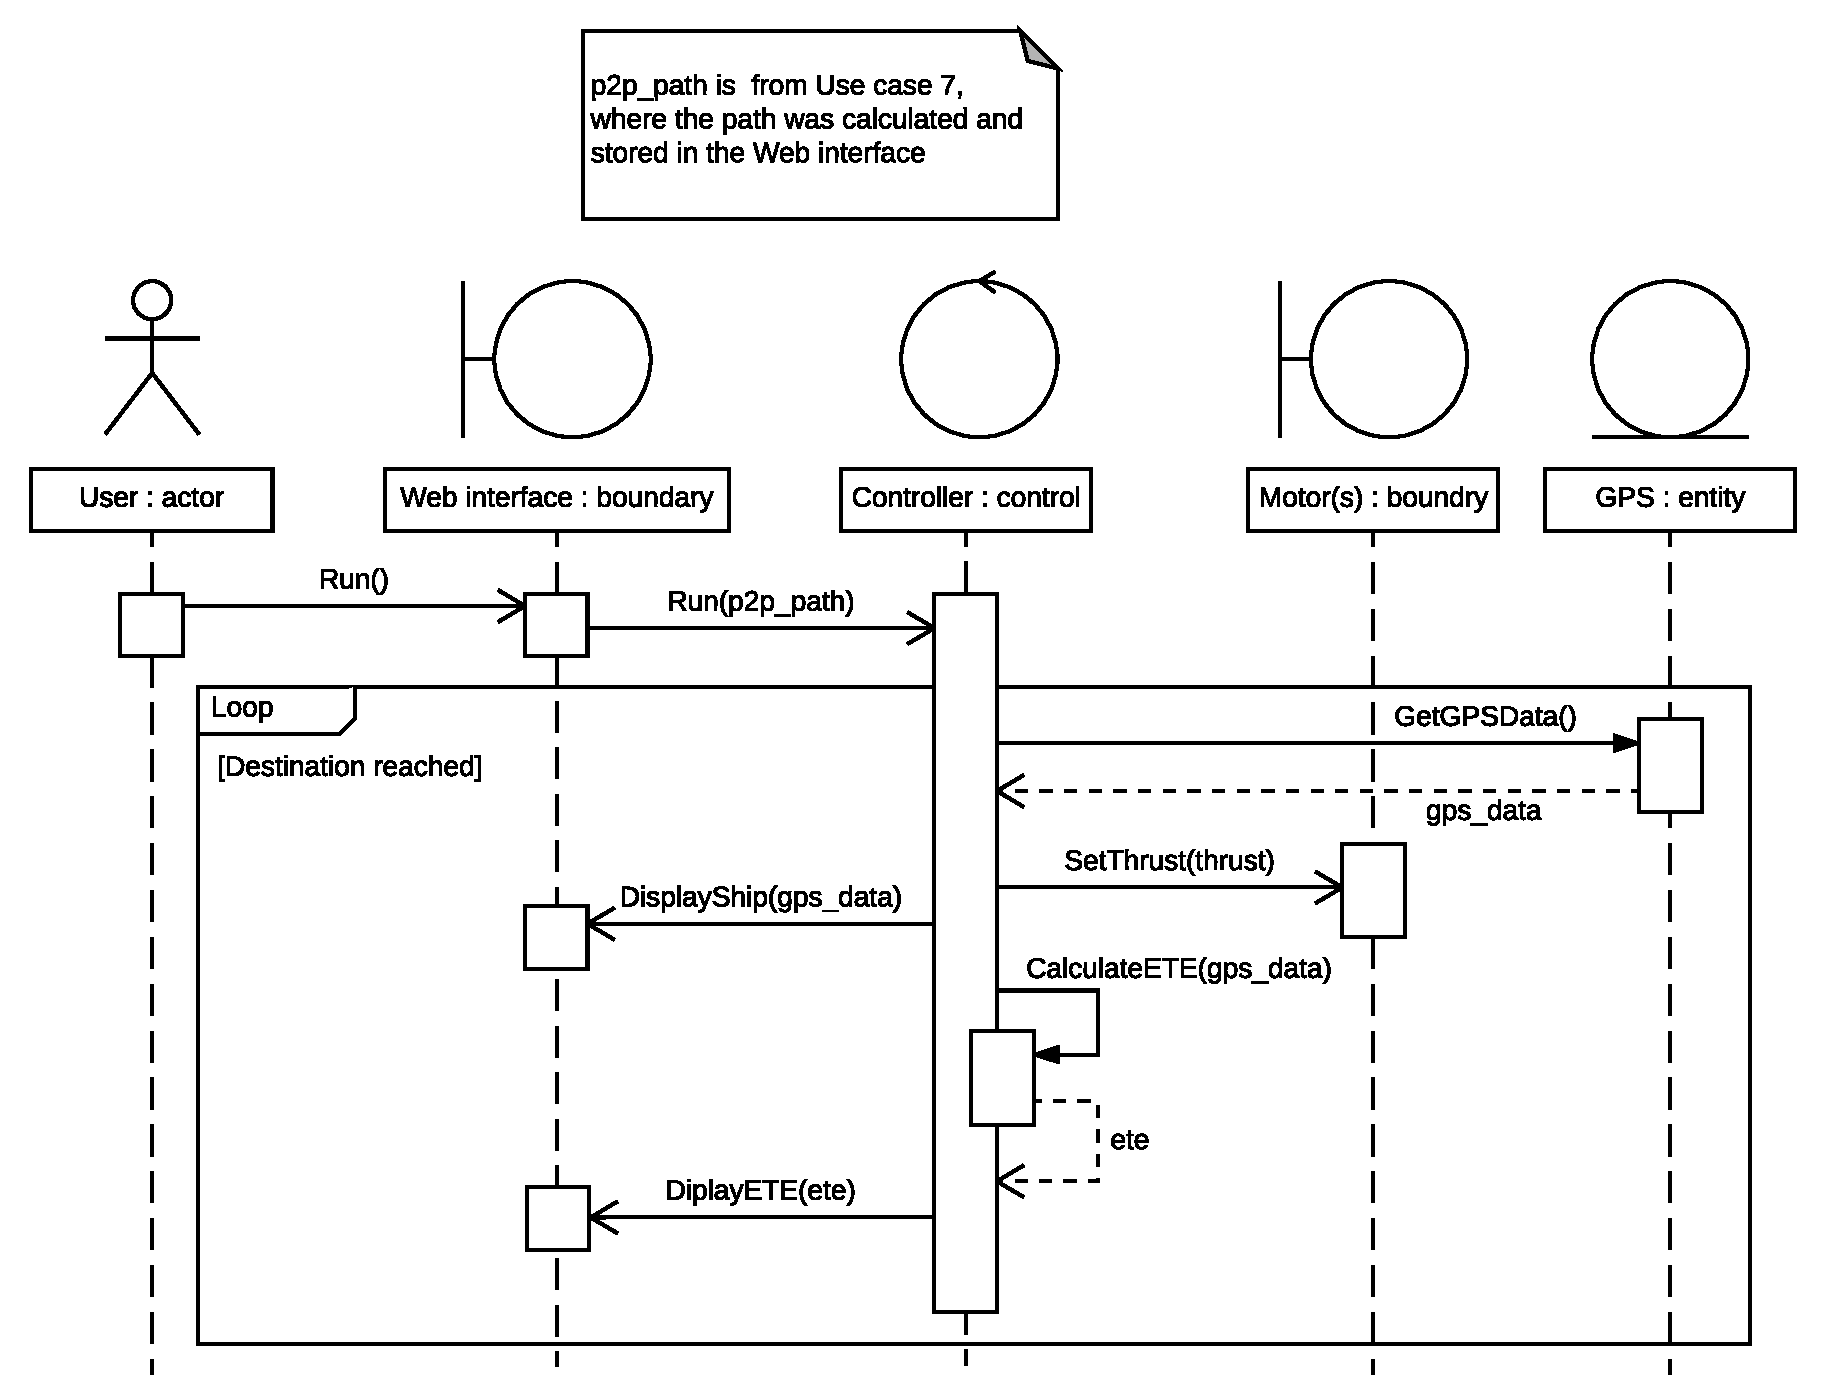
\includegraphics[width=1\linewidth]{Images/System_architecture/Use_case_8_SD}
	\caption{Sequence diagram for Use case 8 - Run point to point path}
	\label{fig:seq:uc8}
\end{figure}

In figure \ref{fig:seq:uc9} the system is already doing the loop from use case 8 as seen on figure \ref{fig:seq:uc8}. But this time a user actor wants to stop the boat, so he calls stop on the web interface this breaks the loop. The web interface relays the stop call to the controller and it set the thrust to 0\% or stopped.

\begin{figure}[H]
	\centering
	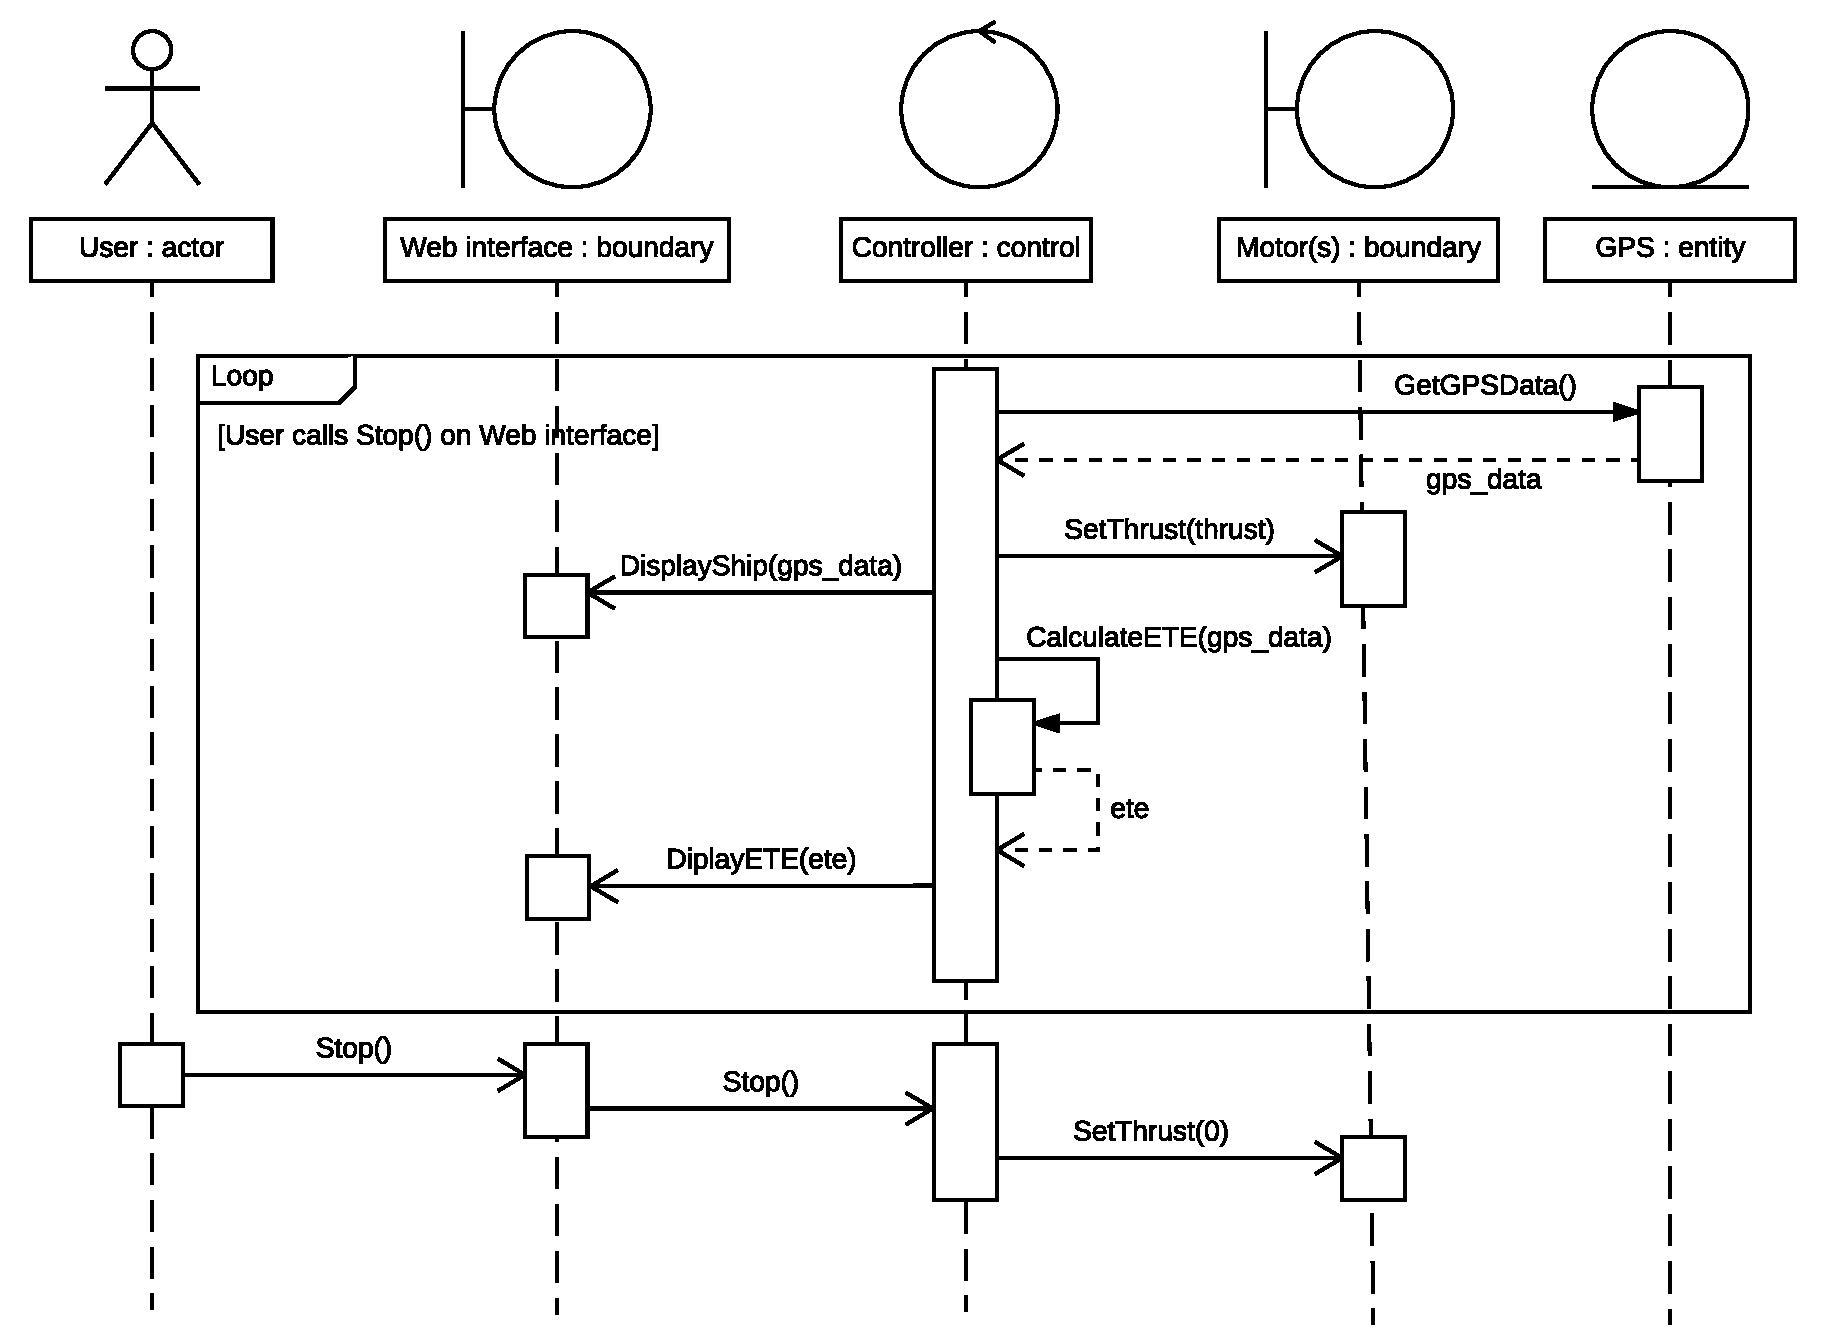
\includegraphics[width=1\linewidth]{Images/System_architecture/Use_case_9_SD}
	\caption{Sequence diagram for Use case 9 - Stop point to point path}
	\label{fig:seq:uc9}
\end{figure}

In figure \ref{fig:seq:uc10} an user actor wants to define a coverage area, he does this with 2 coordinates. The web interface displays the coordinates on a map and as some text as well. 

\begin{figure}[H]
	\centering
	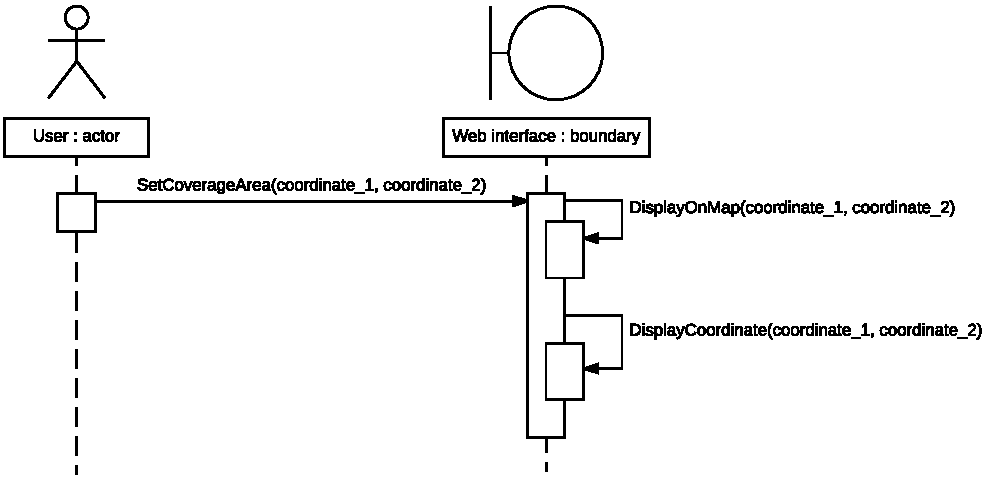
\includegraphics[width=1\linewidth]{Images/System_architecture/Use_case_10_SD}
	\caption{Sequence diagram for Use case 10 - Set coverage area}
	\label{fig:seq:uc10}
\end{figure}

In figure \ref{fig:seq:uc11} a user actor wants to calculate a coverage path, it is a prerequisite that use case 10 has been completed before this so the web interface knows on what to calculate the path. The web interface tells the controller to calculate the path with 2 coordinates defined in use case 8. The controller gets the GPS data to know where the boat is at and returns a calculated path. The web interface then displays the path.

\begin{figure}[H]
	\centering
	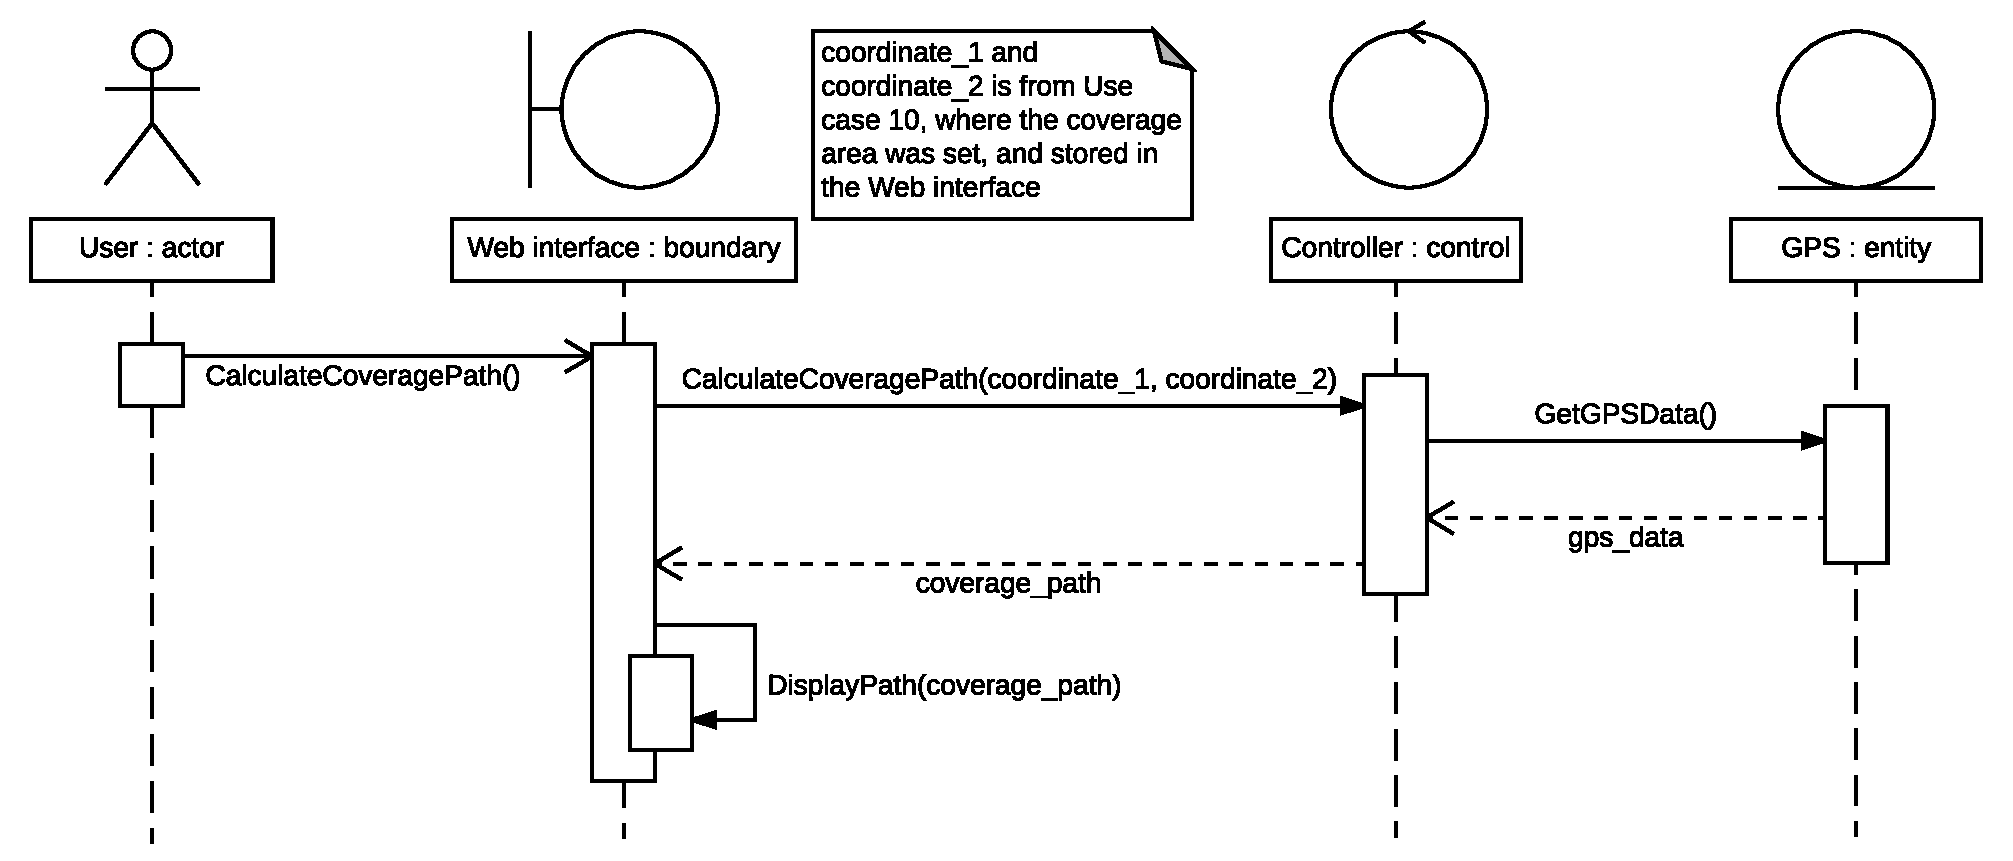
\includegraphics[width=1\linewidth]{Images/System_architecture/Use_case_11_SD}
	\caption{Sequence diagram for Use case 11 - Calculate coverage path}
	\label{fig:seq:uc11}
\end{figure}

In figure \ref{fig:seq:uc12} a user actor wants to run the a coverage path. Before this can be done, first the user must have calculated a path. The web interface tells the controller to run the coverage path previously calculated. The controller now gets the GPS data, and set the thruster(s) accordingly, it then displays the GPS data on the web interface. Then it calculates the estimated time enroute, to display on the web interface. Everything from getting the GPS data is repeated until the destination is reached.

\begin{figure}[H]
	\centering
	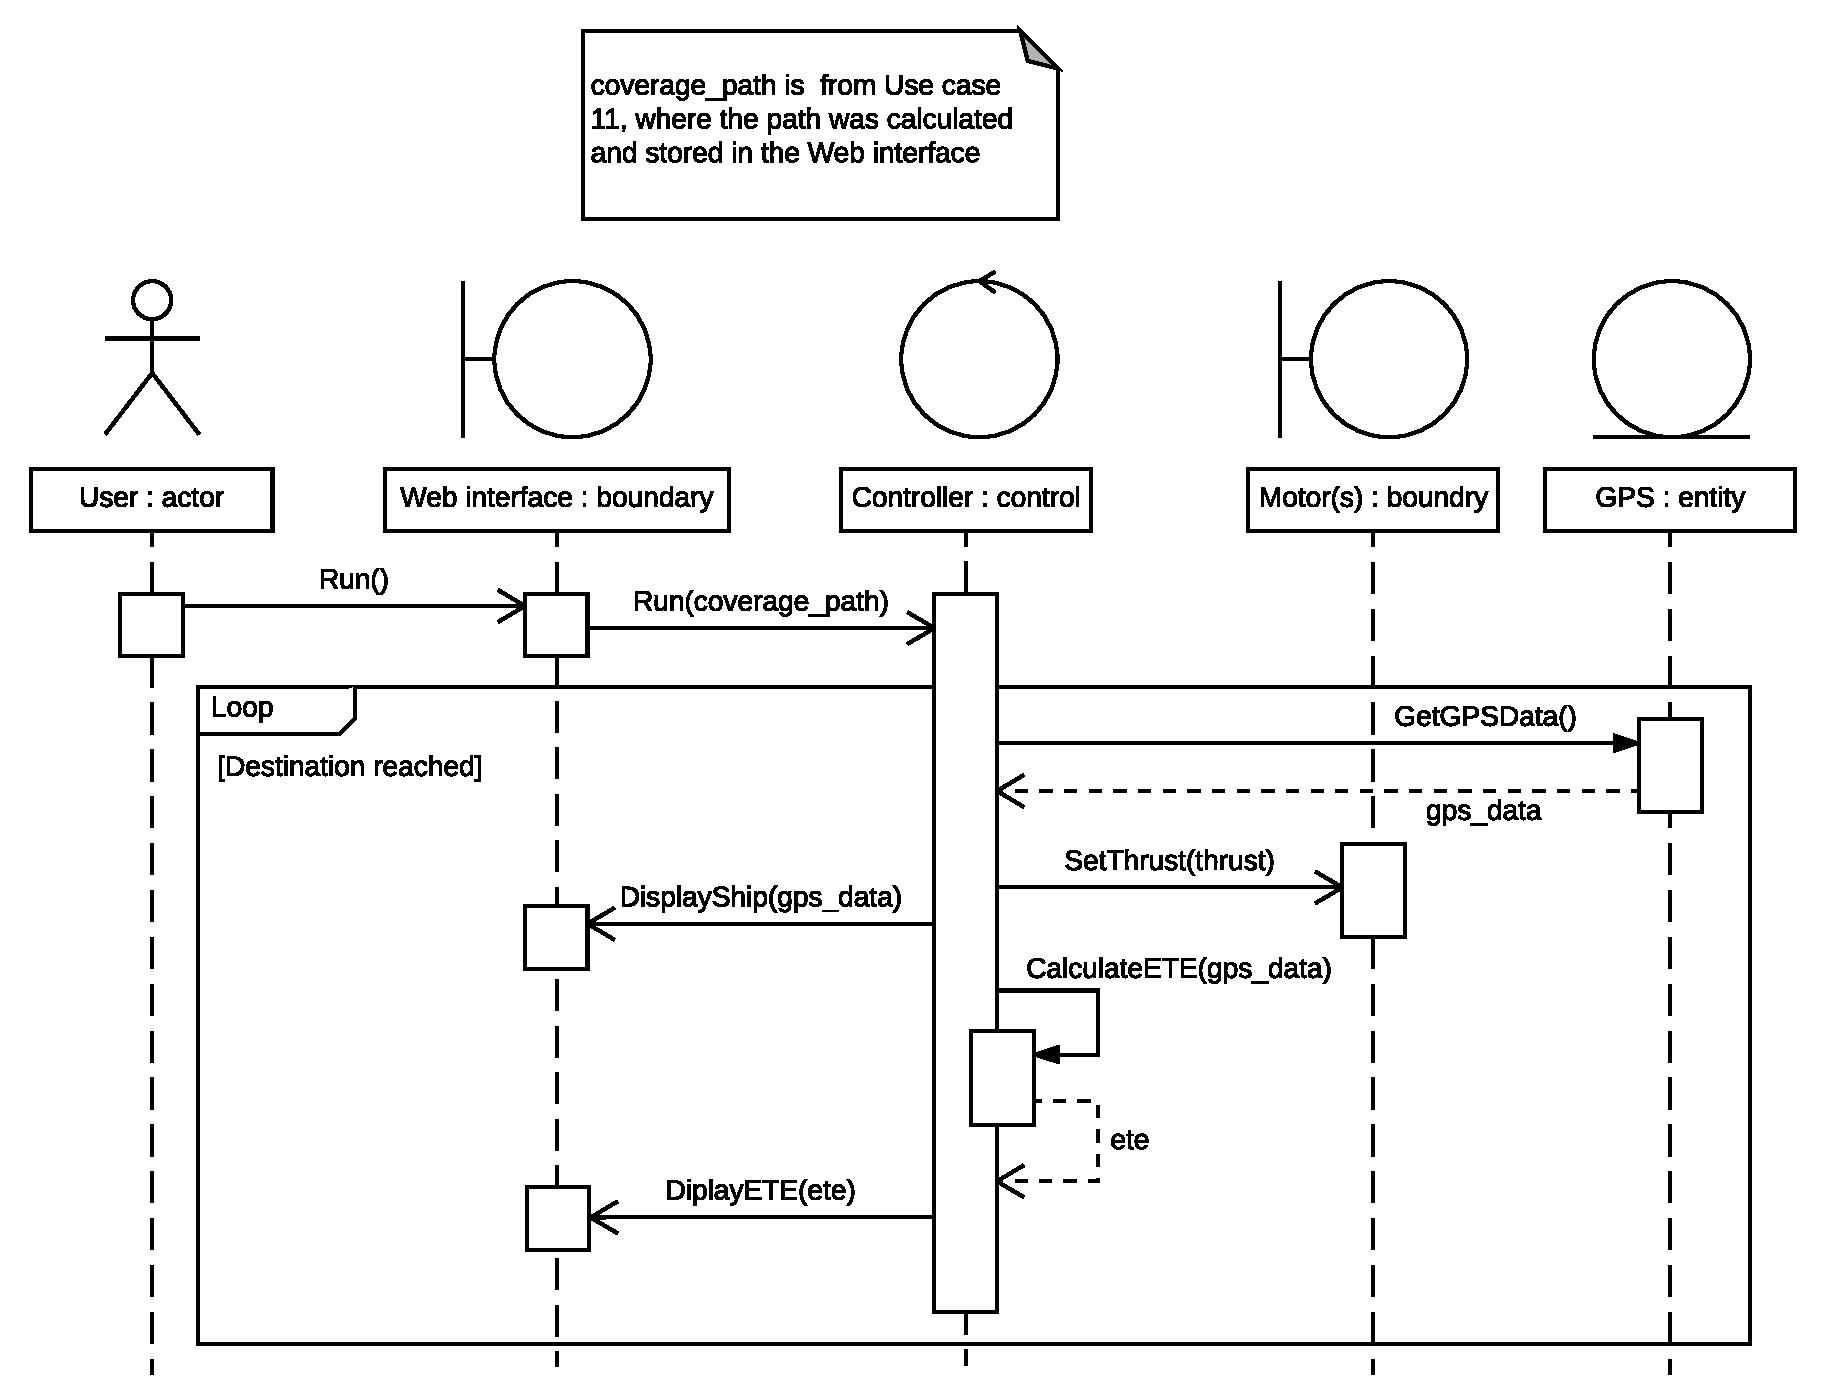
\includegraphics[width=1\linewidth]{Images/System_architecture/Use_case_12_SD}
	\caption{Sequence diagram for Use case 12 - Run coverage path}
	\label{fig:seq:uc12}
\end{figure}

In figure \ref{fig:seq:uc13} the system is already doing the loop from use case 12 as seen on figure \ref{fig:seq:uc12}. But this time a user actor wants to stop the boat, so he calls stop on the web interface this breaks the loop. The web interface relays the stop call to the controller and it set the thrust to 0\% or stopped.

\begin{figure}[H]
	\centering
	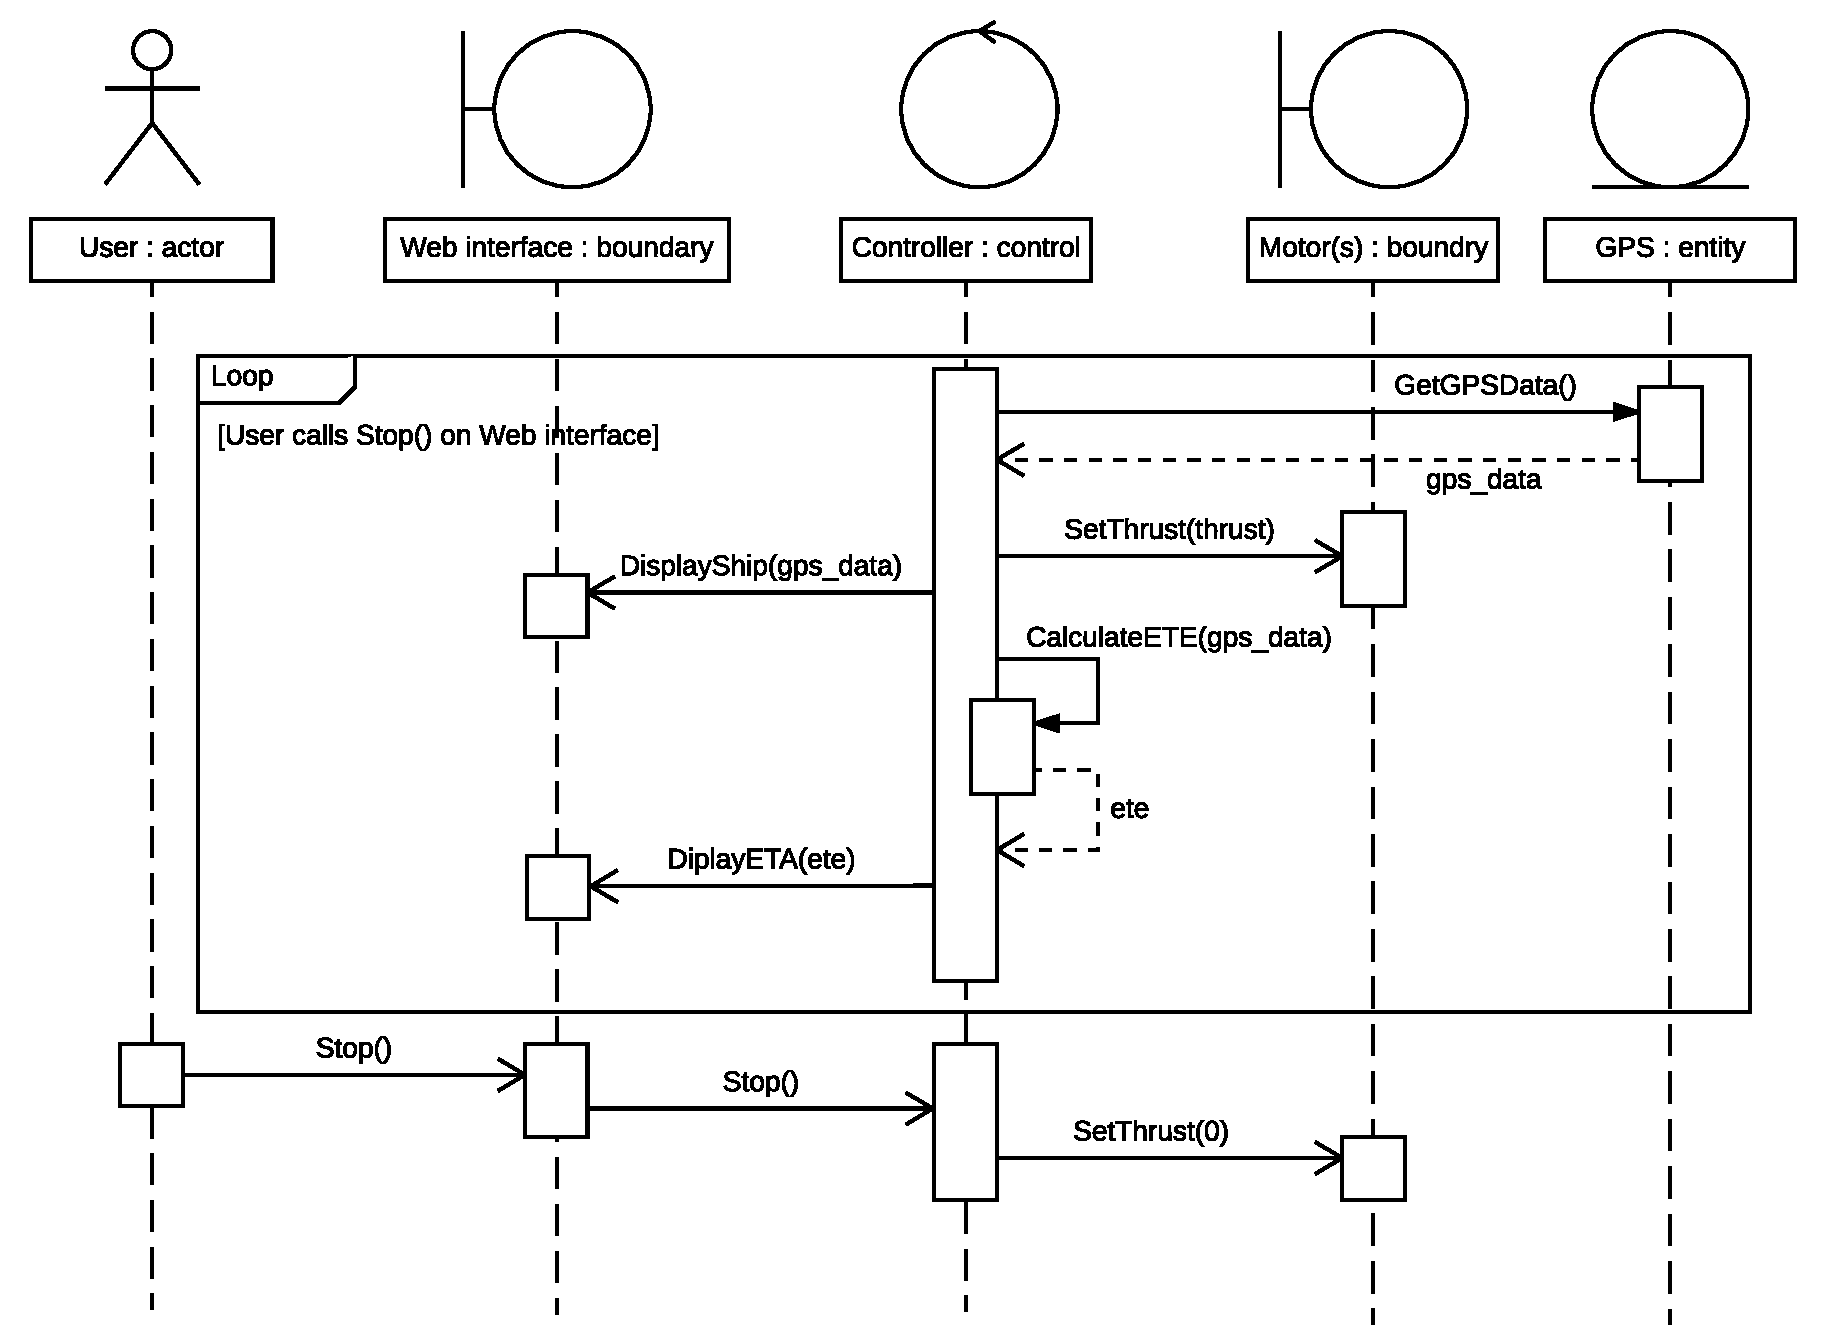
\includegraphics[width=1\linewidth]{Images/System_architecture/Use_case_13_SD}
	\caption{Sequence diagram for Use case 13 - Stop coverage path}
	\label{fig:seq:uc13}
\end{figure}


To summarize the architecture of the system. This system is able to define, calculate and run 2 different paths. It can get different types of diagnostics data. An lastly it can create and manipulate parameter profiles so the system is able to be configured. 




